%=======================+=========================
%================  Simulation  ================
%=================================================
\section[Monte Carlo]{Monte Carlo simulation \label{sec:simulation}}
The detailed simulation of events in the Hall-D beamline and \gx{} detector is performed with a GEANT-based software package. The package was originally developed within the GEANT3 framework~\cite{Brun:1987ma} and then migrated to the GEANT4 framework~\cite{Agostinelli:2002hh,Allison:2016lfl}. The simulation framework uses the same geometry definitions and magnetic field maps as used in reconstruction. The geometry includes the full photon beamline, starting at the radiator and ending at the photon dump. Both internal and external event generators are supported by the framework.  Internal sources include the coherent bremsstrahlung source and the single particle gun. Events read from any number of external generators are also supported. These input events specify one or more primary vertices to be simulated, which are randomized within the hydrogen target with timing that matches the RF structure of the beam.

The Monte Carlo data flow is presented in Fig.~\ref{fig:MC-data-flow}. Events of interest are generated using either an internal or user-supplied event generator. The input event specification is fed to the simulation code, either {\em hdgeant} or {\em hdgeant4}, which tracks the particles through the experimental setup and records the signals they produce in the active elements of the detector. Behavior of the simulation is conditioned by a run number, which corresponds to a particular set of experimental conditions: beam polarization and intensity, beamline and detector geometry, magnetic field maps, etc. All this information is read by the simulation at run-time from the calibrations database, which functions as the single source for all time-dependent geometry, magnetic field, and calibration data relevant to the simulation.

Events written by the simulation are processed by \emph{ mcsmear}, which applies corrections to the simulated hits to account for detector system inefficiencies and resolution, and overlays additional hits from uncorrelated background events. Loss of hits from dead channels, multi-hit truncation, and electronic deadtime are also applied at this step. Information needed for this processing comes from the databases for calibrations and run-conditions, and from files containing real backgrounds sampled using random triggers. Events emerging from the smearing step are deemed to be faithful representations of what the detector would have produced for the given run in response to the specified input. These Monte Carlo events are then processed with the same reconstruction software as used for the real events, and the output is saved to a REST file. These REST files are then made available for physics analysis.

\begin{figure}[t]\centering  
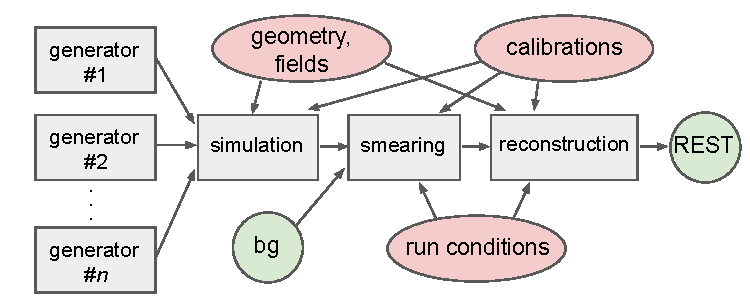
\includegraphics[width=0.95\textwidth]{figures/MonteCarlo_flow.pdf}
\caption[]{\label{fig:MC-data-flow}The Monte Carlo data flow from event generators through physics analysis REST files. The ovals represent databases containing tables indexed by run number, providing a common configuration for simulation, smearing, and reconstruction. Background events represented by the circle marked \emph{bg} are real events collected using a random trigger, which are overlaid on the simulated events to account for pile-up in the Monte Carlo.}
\end{figure}

\subsection[Geometry specification]{\label{sec:materialscan}Geometry specification}
The geometry and material descriptions for the experiment are common across simulation and reconstruction, residing in a family of xml files that follow a common schema called the Hall D Detector Specification, or \emph{HDDS} \cite{HDDS,gx732}. Run-specific variations of the geometry xml records are maintained in the calibration database. The geometry and magnetic field map are also maintained in the calibration database.

The output events from the simulation are written as a data stream, which may either be piped directly into the next step of the Monte Carlo pipeline or saved to a file. Events are passed between 
all stages of the Monte Carlo processing pipeline, shown in Fig.~\ref{fig:MC-data-flow}, using the common data format of the Hall-D Data Model, HDDM \cite{gx65}. HDDM is used for all intermediate input and output event streams.

\subsection{Event generators \label{sec:generators}}
Simulation starts with the generation of events, which can be specific particles or reactions, or simply unbiased background events. A common toolset has been developed to minimize redundancy. These tools include standard methods to generate the distributions of primary photon beam energies and polarization. An output interface is used to produce files suitable as input to the GEANT simulation.

The photon beam energy distribution can be produced using a coherent bremsstrahlung generator that accounts for the physical properties of the radiator and the photon beamline. This generator allows the user to select the orientation of the diamond radiator, and then calculates the linear polarization for each photon. Photons can also be generated according to the spectrum measured in the pair spectrometer during any actual data run by interfacing to the calibration data base. Here the user inputs the degree of linear polarization and the orientation. Finally, the user can provide a histogram of the photon energy spectrum and a second one of the degree of polarization to be used to generate the photon beam. 

One of the first generators was used to simulate the entire photoproduction cross section, and is currently used to study backgrounds to physics reactions as well as develop analysis tools for extracting signals. This event generator, called {\em bggen}, is based on Pythia~\cite{Sjostrand:2006za}, but includes additions that describe the low-energy photoproduction cross sections. Other generators are tied to specific reactions, where the generator needs to describe the underlying physics.

\subsection{HDGEANT \label{sec:hdgeant}}
Both GEANT3 and GEANT4 versions are available for simulation of the experiment. Both versions have been tuned to reproduce the behavior of the experiment, but there are some differences arising from how the two versions decide when to stop tracking particles. In general, the simulation mimics the running conditions found across a range of runs, typically a large part of a single run period. The output from GEANT contains both hit times and energies deposited in detector volumes. 

\subsection[Detector response]{Detector response}
Converting time and energy deposits coming from GEANT into electronic detector responses that match the readout from the experiment is carried out by the detector response package \textit{mcsmear}. The output of this digitization is identical to the real data with the exception that the so-called \emph{truth information} about the data is retained to allow detailed performance studies. In addition to the digitization, at this stage the run-dependent efficiency effects are applied to the data, including both missing electronic channels and reduced efficiency of other channels. Additional smearing of some signals is also applied here to better match the performance of the Monte Carlo to data. 

This detector-response package also folds measured backgrounds into the data stream. During regular data collection, random triggers are collected on a periodic basis during each run. These are separated from the actual data and used to provide experimental background signals in the Monte Carlo, with the rate of random events added based on the actual beam fluxes in the experiment. 

\subsection{Job submission \label{sec:jobsubmission}}
Due to the large number of experimental conditions that need to be matched in simulated data, the \emph{MCWrapper} tool was developed to streamline the input specifications, implement consistency with corresponding data reconstruction, seamlessly access computer offsite resources, and produce Monte Carlo samples in proportion to the actual data taken. The goal is to model the differences between runs and provide a simulated data set, comparable to the real data. The primary system used for this phase is the Open Science Grid (OSG) in order to leverages resources in addition to the local JLab computing farm. Many automatic checks are made to avoid flawed submission, and all aspects of the requests and jobs are monitored during running. Once completed, \emph{MCWrapper} checks for expected output files to be returned as if the jobs were run on the JLab farm. If expected files are not found the system will automatically submit a replacement job. Once the jobs are verified completed and all data from the request has been properly moved, the user receives an automated email alerting them that their request has been fulfilled and the location where the user can access the event sample.

Users are able to monitor and control their simulations via an online dashboard. The \emph{MCWrapper} dashboard gives information about active projects and allows users (or administrators) to interact with their requests. Users may cancel, suspend, or declare projects complete. Detailed information is presented about the individual jobs, such as where the jobs are being run, basic usage statistics, and current status.  This information gives individuals a near real-time look into the production of their Monte Carlo samples.

%Because of the large number of experimental conditions that need to be matched in simulating data, the \emph{MCWrapper} tool has been developed to manage simulations. The tool can be used 'stand-alone' and integrates with various GlueX databases to allow users to run their own individual Monte Carlo workflows in sets of experimental runs with parameters of those runs automatically used.  MCwrapper also provides Monte Carlo samples in proportion to the actual data taken.  In principle this should better model the differences between runs and provide a simulated data set more comparable to the data.  Users who need a Monte Carlo sample can also use a web-based interface (Figure \ref{fig:MCWrapperSubmit} to MCWrapper (MCWrapper-bot) to select the event generator, the version of Geant, the run period of interest and versions of reconstruction and simulation code. This form is dynamic and only presents options to users as needed.  This keep clutter to a minimum and reduces potential confusion when approaching simulation in GlueX. Incorporated into the web form is also a simple web form to properly configure the analysis of produced files from the reconstruction step.  This is done in plain-text as to reduce errors in configuration. Once submitted MCWrapper-bot then correctly configures MCWrapper based on information provided by the user.  Once configured the automated system tests a small sub-sample of the request with the requested software stack.  This attempts to limit flawed submissions to computational resources.  On test failure the submitting user is supplied all logging information and a link that allows them to correct any miss-configuration and flag their project to be retested.  All of this happens without user intervention.  When the test is passed the system breaks the request into a number of jobs and submits the needed jobs to one of several systems.  The primary system used is the Open Science Grid, however the system decides on where to submit the job on a job by job basis. For example, if the system detects a forming backlog on the Open Science Grid, marked in part by a large number of idle jobs, it will seamlessly begin submitting to the local Jefferson Lab computing farm. While running all aspects of the requests and jobs are monitored.  If a job encounters problems MCWrapper-bot will attempt to diagnose it and may even take corrective action automatically (e.g. resubmitting failed jobs that fail for transient reasons). Once completed the system checks for expected files to be returned.  If expected files are not found the system will automatically submit a replacement job. Once the jobs are verified completed and all data from the request has been properly moved, the user receives an automated email alerting them to the fact that their request has been fulfilled and the location where the user can access the event sample.\newline

%Users are able to monitor projects as well as control their projects via an online dashboard (Figure \ref{fig:MCWrapperDashboard}).  The MCWrapper dashboard gives information about active projects and allows users (or administrators) to interact with their requests by right-clicking on the individual row.  Users may cancel, suspend, or declare projects complete. By left-clicking on a row more detailed information is presented including the individual jobs, where the jobs are being run, basic usage statistics of the jobs, and current status.  Users may also see news or notices of outages regarding MCWrapper-bot.  These news articles are dynamically pushed to people on the web page and do not require a browser refresh to obtain.  Not shown are plots of the total number of running and idle jobs from the submit node (a measure of the health and load of the system). Also not shown are the heart beats of the subsystems of MCWrapper-bot with the system the last job was submitted to.  All information on the dashboard is dynamically updated in near real-time.  This gives individuals a near real-time look into the production of their Monte Carlo samples.
%\begin{figure}[h!]\centering
%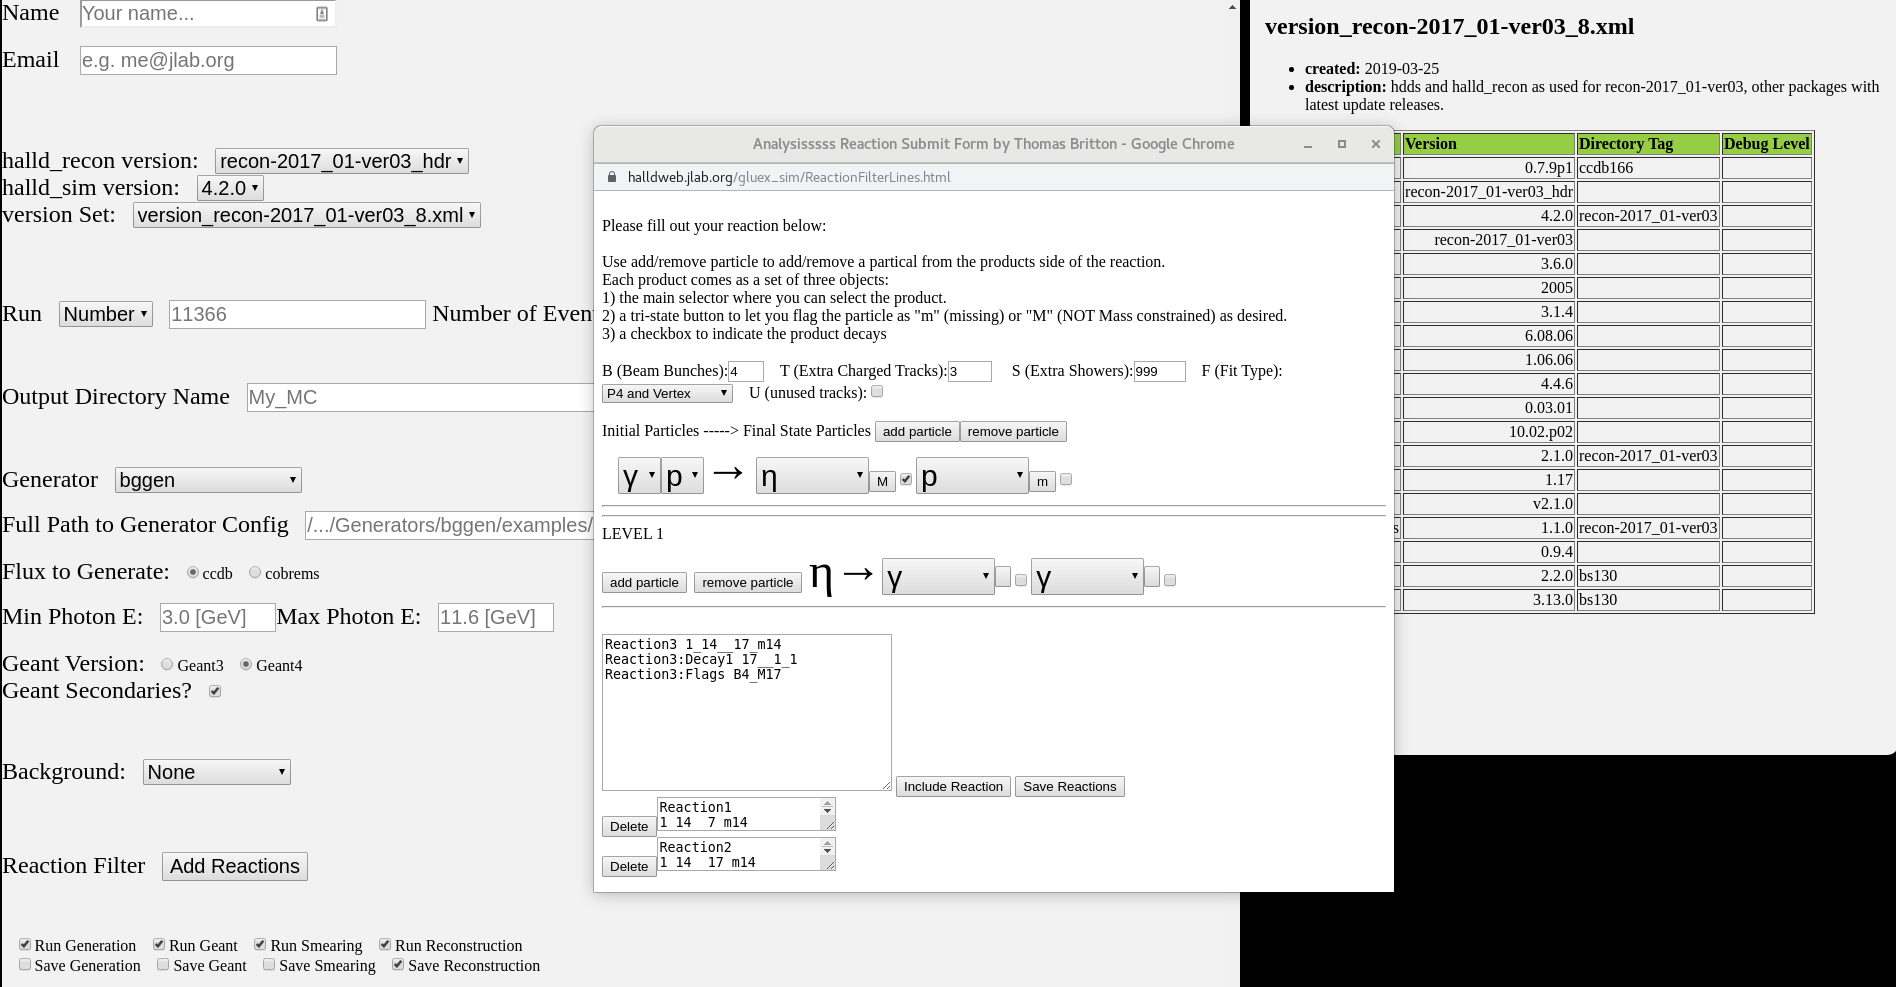
\includegraphics[width=0.85\textwidth]{figures/mcwrapper_submit_form.png}
%\caption{Shown is a section of the web interface where users can request the various configuration parameters including the desired reactions to be analyzed.  The form dynamically generates options as %needed}{\label{fig:MCWrapperSubmit}}
%\end{figure}
%\begin{figure}[h!]\centering
%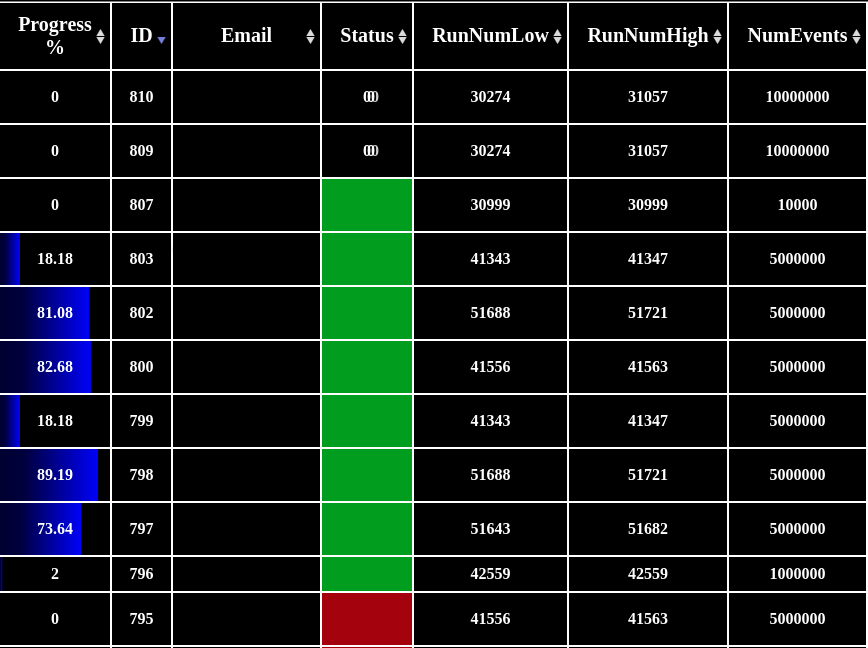
\includegraphics[width=0.85\textwidth]{figures/mcwrapper_dashboard_redacted.png}
%\caption{Shown is a section of the main table of the MCWrapper dashboard with user email addresses redacted. The table provides useful information to users including the current level of completion, the status of the project (green for successfully tested, red for failed tests, and animated ellipses for project currently in testing).  }{\label{fig:MCWrapperDashboard}}
%\end{figure}